\documentclass[main.tex]{subfiles}

\begin{document}
\section{Sviluppo}\label{sec:sviluppo}
\subsection{Come funziona un Ray Tracer}

\begin{minipage}{0.6\textwidth}
\hspace*{0.25in}Il sistema di coordinate adottato per il Ray Tracing è comunemente uno spazio tridimensionale, come illustrato nella Figura 2. In questo spazio, il mondo della scena è posizionato nella parte negativa dell'asse z e viene riflessa nella \textit{viewport} attraverso la camera in modo speculare.
\end{minipage}%
\begin{minipage}{0.4\textwidth}
    \centering
    \fbox{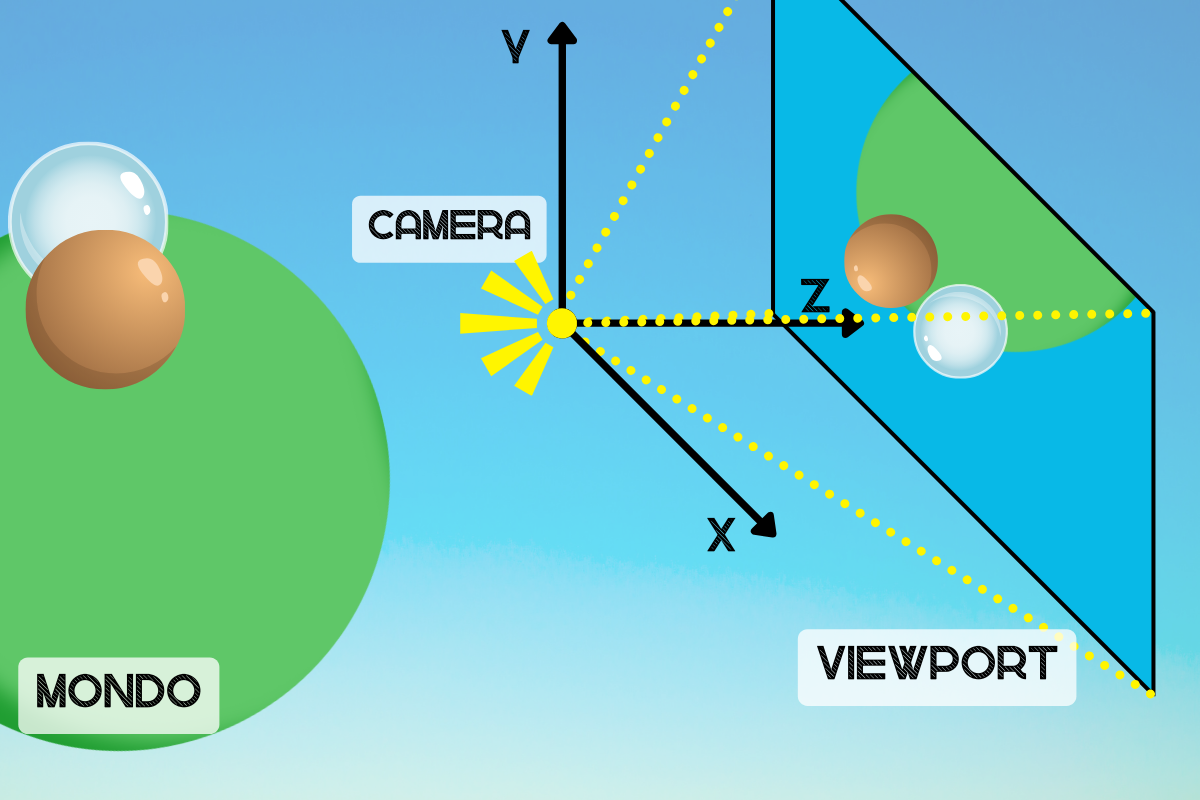
\includegraphics[width=0.9\textwidth]{figures/Coord_Teoriche2.0.png}}
    \captionsetup{aboveskip=0pt}
    \captionof{figure}{Coordinate Teoriche}\vspace{-14pt}\rule{0.9\linewidth}{0.4pt}
\end{minipage}\\
\begin{minipage}{0.4\textwidth}
    \centering
    \fbox{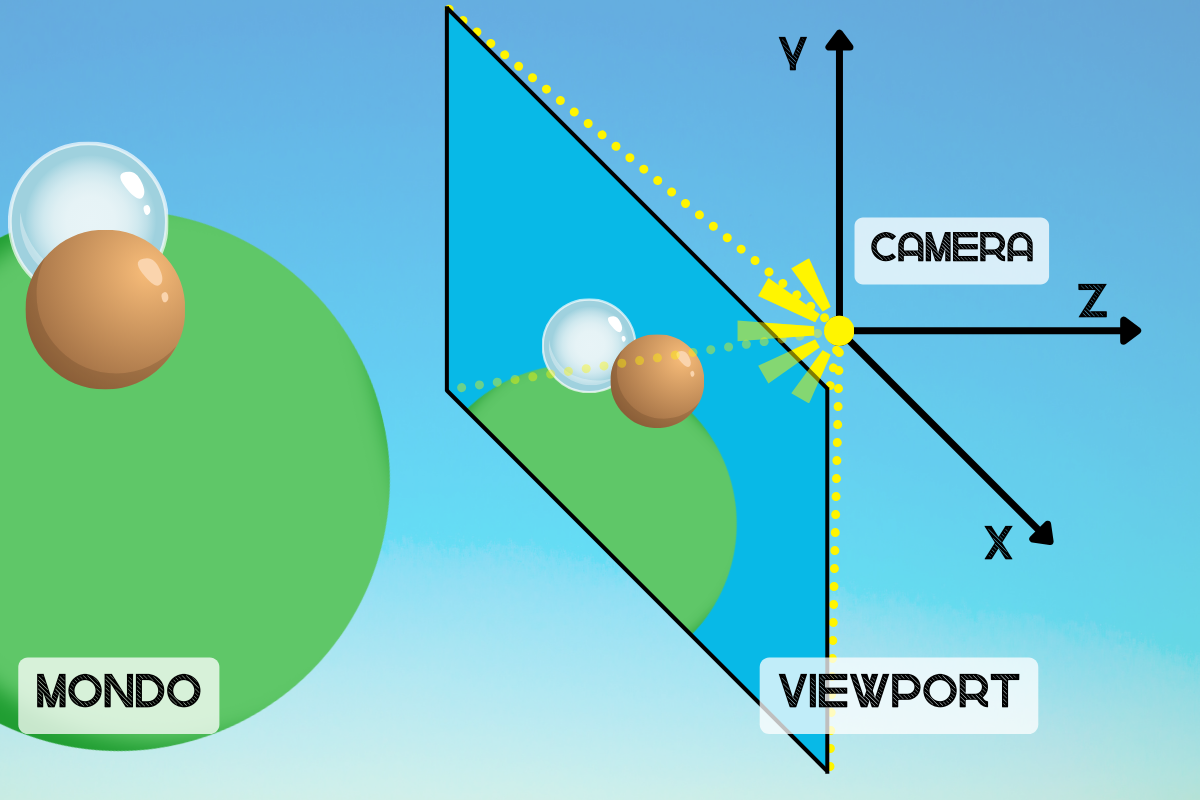
\includegraphics[width=0.9\textwidth]{figures/Coord_Pratiche2.0.png}}
    \captionsetup{aboveskip=0pt}
    \captionof{figure}{Coordinate Pratiche}\vspace{-14pt}\rule{0.9\linewidth}{0.4pt}
\end{minipage}%
\begin{minipage}{0.6\textwidth}
Tuttavia, per semplificare i calcoli, nella pratica si sposta la viewport nella parte negativa dell'asse z, come mostrato nella Figura 3. In questo contesto, un raggio è rappresentato come un vettore con origine nella camera e direzione lungo il segmento che congiunge il pixel associato al raggio con la camera stessa: \(\Vec{Ray} = \Vec{pxl} - \Vec{Cam}\).
\end{minipage}\\\\
Nel codice, la generazione dei raggi è modellata in modo analogo:
\begin{lstlisting}[style=cppstyle, label=cppexample]
ray r(cam_O, lower_left_corner + u*width + v*height - cam_O);
\end{lstlisting}
Una volta generato il raggio, che possiamo scrivere come \(\Vec{R}(t) = \Vec{O} + t\Vec{D}\) in cui \(\Vec{O}\) è \\ 
\begin{minipage}{0.6\textwidth}
 l'origine e \(\Vec{D}\) la direzione, si vanno a calcolare le intersezioni con tutti gli oggetti presenti nel mondo, entro un certo intervallo limite.
Tra tutti i valori \(t\ap{*}\) trovati, si considera il minimo, \(t_{min}\), che rappresenta il punto di intersezione più vicino alla camera: \(\Vec{R}(t_{min})\) è dunque il punto di interesse nello spazio. In base all'oggetto colpito, il raggio si comporta in modo diverso.
\end{minipage}%
\begin{minipage}{0.4\textwidth}
    \centering
    \fbox{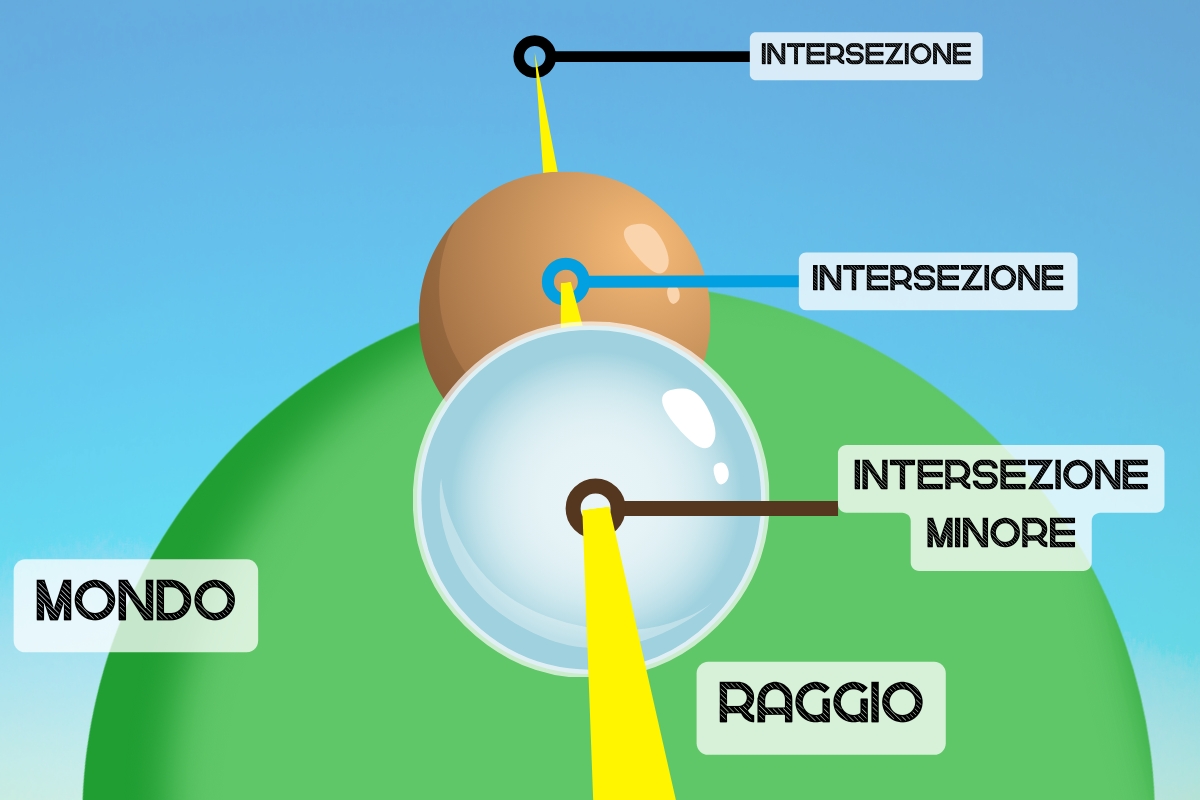
\includegraphics[width=0.9\textwidth]{figures/Intersezioni2.0.png}}
    \captionsetup{aboveskip=0pt}
    \captionof{figure}{Intersezioni}\vspace{-14pt}\rule{0.7\linewidth}{0.4pt}
\end{minipage}\\


Gli oggetti possono assumere forme, materiali e colori diversi.
La forma determina l'equazione da risolvere nel calcolo dell'intersezione: la più semplice è quella della sfera. 
\[
(x - C_x)^2 + (y - C_y)^2 + (z - C_z)^2 = r^2
\]
Sostituendo ad x, y e z le coordinate del raggio variabili in t troviamo l'equazione quadratica da risolvere per trovare l'intersezione 
\[
(\Vec{R}(t) - \Vec{C}) \cdot (\Vec{R}(t) - \Vec{C}) = r^2
\]
Il materiale determina, invece, la modalità di diffusione (\textit{scatter}) del raggio che lo ha colpito. Quelli trattati sono:
\begin{itemize}
    \begin{minipage}{0.54\textwidth}
        \item Metallo: produce una riflessione speculare del raggio rispetto alla normale dell'oggetto. 
        \item Opaco: produce una riflessione diffusa del raggio, ovvero non lungo la direzione speculare, ma lungo direzioni casuali. Un diffusore ideale è detto lambertiano e riflette la luce omogeneamente in tutte le direzioni. 
        \end{minipage}%
    \begin{minipage}{0.4\textwidth}
        \centering
        \fbox{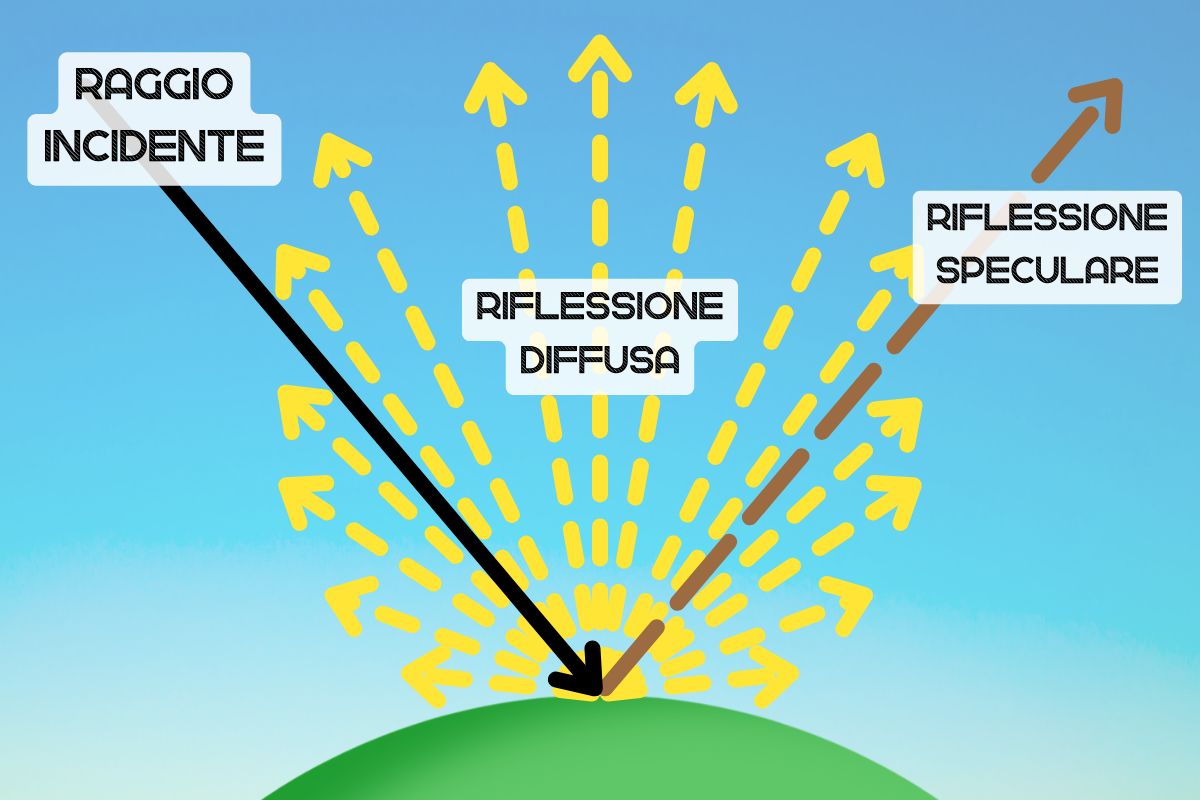
\includegraphics[width=0.9\textwidth]{figures/riflessione.png}}
        \captionsetup{aboveskip=0pt}
        \captionof{figure}{Riflessione}\vspace{-14pt}\rule{0.65\linewidth}{0.4pt}
    \end{minipage}
    \item Vetro: nei dielettrici il raggio si sdoppia in una componente riflessa e una rifratta. Abbiamo semplificato il concetto scegliendo casualmente una delle due componenti da diffondere per evitare di avere tempi di computazione esponenziali. 
\end{itemize}
Infine, il colore determina il potere riflettente di un oggetto (\textit{albedo}). Di fatti, più un oggetto tende al bianco \textit{(1,1,1)}, più tenderà a riflettere i colori degli oggetti vicini; più tende al nero \textit{(0,0,0)}, e più assorbirà i colori. Questo comportamento è ottenuto moltiplicando, per ogni pixel, i colori degli oggetti intersecati dal raggio associato durante le riflessioni e rifrazioni. 
Da notare che quando il raggio non interseca nulla assorbe il colore dello sfondo, mentre quando rimbalza molte volte tra vari oggetti si genera un colore scuro: un'ombra. \\
\begin{minipage}{0.4\textwidth}
    \centering
    \fbox{
\includegraphics[width=0.9\textwidth]{figures/aliasing.png}}
    \captionsetup{aboveskip=0pt}
    \captionof{figure}{Aliasing}\vspace{-14pt}\rule{0.6\linewidth}{0.4pt}
\end{minipage}%
\begin{minipage}{0.6\textwidth}
  \hspace*{0.25in}Ora, nonostante sia posta un'alta definizione, si nota una certa discontinuità nell'immagine. Ciò è dovuto all'effetto aliasing, che rende l'immagine ben lontana dalla realtà a cui siamo abituati in cui i contorni sono influenzati dai colori vicini. La tecnica di antialiasing consiste nel campionare (\textit{sampling}) ogni pixel generando più raggi con direzioni lievemente modificate. 
\end{minipage}\\\\
Il colore associato a ciascun pixel è la media ponderata dei colori restituiti da questi raggi, rendendo l'immagine più realistica all'aumentare del numero di campioni.

Infine, bisogna considerare la possibilità di spostare la camera ed utilizzare degli effetti avanzati. 
Lo spostamento della camera viene ottenuto eseguendo dei cambi di coordinate e riposizionando la viewport. 
%viewport_upper_left = center - (focal_length * w) - viewport_u/2 - viewport_v/2;
% con viewport_u / _v che puntano dove puntano gli indici i e j per costruzione
Altezza e larghezza di quest'ultima sono dipendenti dal parametro \textit{vfov (Vertical Field of View)} che permette di regolare lo zoom.  
			% theta = vfov * float(M_PI) / 180.0f;
			% half_height = tan(theta / 2.0f);
			% half_width = aspect * half_height;
Con i parametri di \textit{apertura} e \textit{distanza focale} è possibile riprodurre la messa a fuoco: maggiore è l'apertura, maggiore sarà la sfocature dell'immagine. Per ottenere questo effetto, durante la generazione di un raggio, anziché prendere come origine il centro della camera, si seleziona un punto casuale in un suo intorno, definito in modo proporzionale all'apertura.
\begin{lstlisting}[style=cppstyle, label=cppexample]
ray get_ray(...) {
    vec3 r = rnd_in_disk() * cam->aperture / 2.0f;
    return (ray(cam->origin + dot(cam->axis, r), ...)); }
\end{lstlisting}
%     func get_ray(...) {
%           vec3 rd = rnd_in_disk() * this->lens_radius;
% 			offset = this->u * rd.x() + this->v * rd.y();
% 			return (ray(this->origin + offset, ...);

\subsection{Parallelizzazione del Codice}
% metodologia foster
La gestione di una lunga lista di oggetti all'interno del mondo può comportare tempi di esecuzione eccessivamente prolungati. In questo contesto, la parallelizzazione emerge come un elemento chiave, sfruttando la collaborazione tra threads al fine di accelerare l'esecuzione del programma. \\
Per affrontare questa sfida, abbiamo adottato la \textit{Metodologia Foster} \cite{Foster}, che ci ha permesso di costruire uno schema generale del programma con i seguenti passi:
\begin{enumerate}
    \item \textbf{Partizionamento}: abbiamo identificato le attività suscettibili di parallelizzazione, come la generazione dei raggi, il calcolo delle intersezioni lungo la loro traiettoria e la determinazione del colore associato a un pixel specifico.
    
    \item \textbf{Comunicazione}: è necessario che le attività ricevano le informazioni sul mondo e i dati relativi alla camera per eseguire i calcoli. Al termine, è essenziale che comunichino i risultati ottenuti. Inoltre, attività che agiscono sullo stesso raggio devono condividere i dati ad esso relativi.
    
    \item \textbf{Agglomerazione}: per ridurre eccessive comunicazioni e ottimizzare le operazioni, è possibile aggregare le attività relative a un singolo raggio. Un'attività può così gestire la generazione del raggio, la diffusione e il calcolo del colore da restituire. 
    
    \item \textbf{Mappatura}: considerando che le attività da eseguire sono simili e devono essere ripetute su molti dati diversi, viene logico adottare un hardware di tipo \textit{SIMD (Single Instruction Multiple Data)} \cite{flynn} come le GPU. Ognuna di queste attività, infatti, può essere eseguita da un \textit{CUDA thread} tramite un kernel. L'\textit{host} sarà responsabile di inviare i dati corretti e recuperare i risultati ottenuti.
    
\end{enumerate}

Per implementare queste fasi, ci siamo ispirati a un articolo sul blog \textit{NVIDIA}\cite{rtCUDA} che tratta le stesse tematiche. Di base, il flusso del programma coinvolge l'inizializzazione delle memorie, la chiamata al kernel di rendering e la copia del buffer dell'immagine prima sull'\textit{host} e successivamente su file. \\
L'\textit{host} si occupa di allocare sulla memoria del \textit{device} il mondo e la camera. Di conseguenza, il kernel di creazione del mondo viene chiamato per inizializzare la lista di oggetti e la camera direttamente sulla memoria del dispositivo. \\
% TODO: {se avanza spazio} codice con cudaMalloc e createWorld<<<>>>
Inizia quindi la fase cruciale: viene chiamato il kernel di rendering, assegnando un thread a ogni pixel dell'immagine. Dopo aver calcolato il proprio ID, ogni thread genera un numero prestabilito di raggi, affidandosi ai valori della camera. Il thread calcola l'intersezione con l'oggetto più vicino, tenendo conto della diffusione e del colore colpito. Questi fattori determinano la nuova direzione di propagazione e l'attenuazione del raggio. I colori dei raggi campionati vengono mediati e applicati al buffer dell'immagine. \\
% TODO: {se avanza spazio} codice del sampling
Al termine delle operazioni, la memoria utilizzata viene liberata attraverso un kernel apposito e le classiche funzioni di deallocazione. Infine, l'\textit{host} si occupa di generare l'immagine, copiando su file il buffer restituito dal kernel di rendering. 
% TODO: {se avanza spazio} free e free_world


\end{document}